\documentclass[12pt]{article}
%\usepackage{snapshot}  % Creates .dep file showing dependencies
\usepackage[a4paper, margin=0.5in]{geometry}

\usepackage{anyfontsize}
\usepackage{xcolor}
\usepackage{graphicx}
\usepackage{setspace}
\usepackage{hyperref}
\usepackage{booktabs}
\usepackage[backend=biber]{biblatex}
\usepackage{float}
\usepackage{siunitx}
\usepackage{svg}
\usepackage{xepersian}
\usepackage{algorithm2e}
\usepackage{caption}
\usepackage{amssymb}
\usepackage{amsmath}
\usepackage{enumitem}
\usepackage{bigints}
\hypersetup{colorlinks,urlcolor=blue}
%\settextfont[Scale=1.1]{Far.Mitra}

\settextfont[Scale=1.0, Size=14pt]{B Nazanin}
\defpersianfont\persiantitlefont[Scale=1.0, Size=18pt]{B Titr}
\setlatintextfont[Scale=1.0, Size=12pt]{Times New Roman}
\deflatinfont\englishtitlefont[Scale=1.0, Size=16pt]{Times New Roman Bold}

\usepackage[backend=biber]{biblatex}
\addbibresource{references.bib}


\def\labelitemi{$\diamond$}
\def\labelitemii{$\ast$}
\setcounter{secnumdepth}{0}  % Depth 0 = no section numbering

\begin{document}
	\linespread{3}
	\setstretch{1.5}
	
	% --- HEADER ROW ---
	\begin{minipage}[t]{0.7\textwidth}
		\huge\textcolor{teal!70!black}{\title\textbf{{استنباط آماری}}}
	\end{minipage}
	\hfil
	\begin{minipage}[t]{0.15\textwidth}
		\centering
		
\includegraphics[width=0.9\linewidth]{pics/logo.png}\\[6pt]
		{\small پاییز ۱۴۰۴}
	\end{minipage}
	
	
	
	{
		
		\Large{تمرین سوم}
		
		\large مرتضی ملکی‌نژاد شوشتری - ۸۱۰۱۰۴۲۵۶
		
		
	}
	
	\vspace{1.2cm}
	
	
	
	\vspace{0.3cm}
	\hrule
	\vspace{0.6cm}
%	\tableofcontents


\section{پاکسازی داده و استخراج ویژگی}

\subsection{داده‌های اولیه}
مجموعه داده شامل ۷۲۰ فایل صوتی است که به صورت زیر توزیع شده‌اند:
\begin{itemize}
	\item زبان آلمانی: ۱۸۰ نمونه
	\item زبان ایتالیایی: ۱۸۰ نمونه
	\item زبان کره‌ای: ۱۸۰ نمونه
	\item زبان اسپانیایی: ۱۸۰ نمونه
\end{itemize}

همه فایل‌های صوتی با نرخ نمونه‌برداری \lr{16} کیلوهرتز بارگذاری شده‌اند.

\subsection{استخراج ویژگی‌ها}
برای استخراج ویژگی‌های مناسب از فایل‌های صوتی، از دو روش اصلی استفاده شده است:

\subsubsection{ویژگی‌های \lr{MFCC}}
\lr{MFCC (Mel-Frequency Cepstral Coefficients)} یکی از ویژگی‌های رایج در پردازش سیگنال‌های صوتی است که اطلاعات مهمی در مورد طیف فرکانسی سیگنال ارائه می‌دهد. در این پروژه، \lr{13} ضریب \lr{MFCC} برای هر فایل صوتی استخراج شده است.

\subsubsection{ویژگی‌های \lr{Mel Spectrogram}}
\lr{Mel Spectrogram} نمایشی از انرژی سیگنال در مقیاس \lr{Mel} است که به درک انسان از فرکانس نزدیک‌تر است. در این پروژه، \lr{128} ویژگی \lr{Mel Spectrogram} برای هر فایل صوتی استخراج شده است.

چون طول صوت‌ها برابر نیست، بعد دوم این ویژگی‌ها متفاوت است. و اکثر الگوریتم‌هایی که در ادامه استفاده می‌شوند نیاز دارند تا ابعاد ویژگی‌ها ثابت باشد. به همین منظور از این ویژگی‌ها در بعد دوم میانگین گرفته شد. 
\subsubsection{ترکیب ویژگی‌ها}
در نهایت، با ترکیب این دو مجموعه ویژگی، یک بردار ویژگی \lr{141} بعدی برای هر نمونه ایجاد شده است:
\begin{equation}
X_{combined} = [X_{MFCC}, X_{Mel}]
\end{equation}
که در آن $X_{MFCC} \in \mathbb{R}^{13}$ و $X_{Mel} \in \mathbb{R}^{128}$ هستند.

\subsection{نرمال‌سازی}
برای بهبود عملکرد الگوریتم‌های یادگیری ماشین، تمام ویژگی‌ها با استفاده از \lr{StandardScaler} نرمال‌سازی شده‌اند تا میانگین صفر و واریانس واحد داشته باشند.

\subsection{تجسم داده‌ها}
برای تجسم بهتر داده‌ها، از تحلیل مؤلفه‌های اصلی (\lr{PCA}) استفاده شده و داده‌ها در فضای دو بعدی نمایش داده شده‌اند. شکل \ref{fig:pca_features} نمایش \lr{PCA} ویژگی‌های \lr{MFCC} و \lr{Mel Spectrogram} را نشان می‌دهد.

\begin{figure}[H]
	\centering
	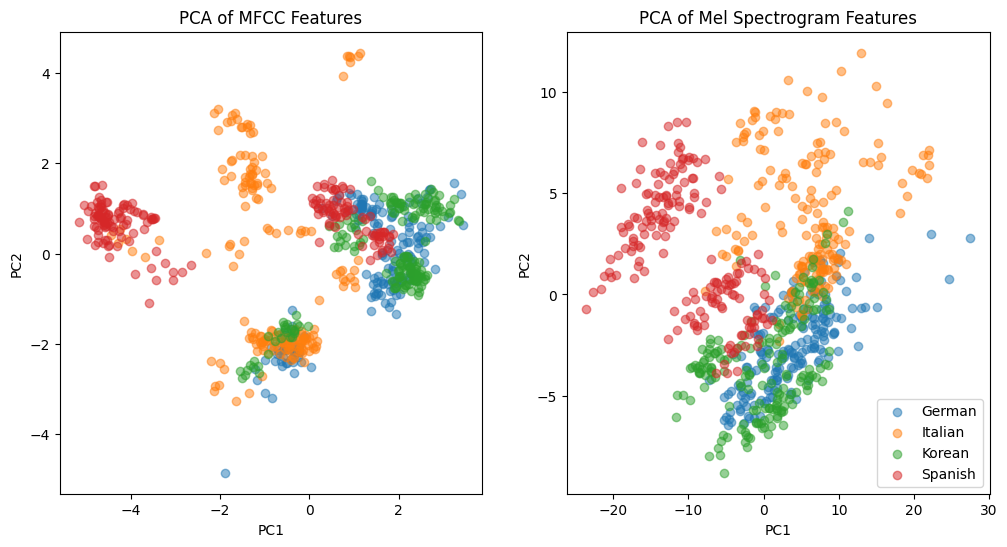
\includegraphics[width=0.9\textwidth]{pics/pca_features.png}
	\caption{نمایش \lr{PCA} ویژگی‌های \lr{MFCC} و \lr{Mel Spectrogram}}
	\label{fig:pca_features}
\end{figure}

\section{خوشه‌بندی}

\subsection{تعیین تعداد خوشه‌های بهینه}
برای تعیین تعداد خوشه‌های بهینه، از دو روش استفاده شده است:
\begin{itemize}
	\item روش \lr{Elbow}: بررسی تغییرات \lr{Within Cluster} نسبت به تعداد خوشه‌ها
	\item روش \lr{Silhouette Score}: محاسبه نمره \lr{Silhouette} برای تعداد خوشه‌های مختلف
\end{itemize}

نتایج حاصل از این دو روش در جدول \ref{tab:optimal_clusters} و شکل \ref{fig:optimal_clusters} نمایش داده شده‌اند.

\begin{table}[H]
	\centering
	\caption{نتایج تعیین تعداد خوشه‌های بهینه}
	\label{tab:optimal_clusters}

	\begin{tabular}{ccc}
		\toprule
		تعداد خوشه‌ها & \lr{within cluster sum} & \lr{Silhouette Score} \\
		\midrule
		۲ & $0.3052$ & $68106.60$  \\
		۳ & $0.2814$ & $52850.66 $\\
		۴ & $0.2558$ & $46053.22$ \\
		۵ & $0.2550$ & $41255.80$ \\
		۶ & $0.2570$ & $36803.24$ \\
		۷ & $0.2805$ & $32713.95$ \\
		۸ & $0.2937$ & $30534.69$ \\
		۹ & $0.2966$ &$28647.57$ \\
		۱۰ & $0.2971$ & $26826.33$ \\
		\bottomrule
	\end{tabular}

\end{table}

\begin{figure}[H]
	\centering
	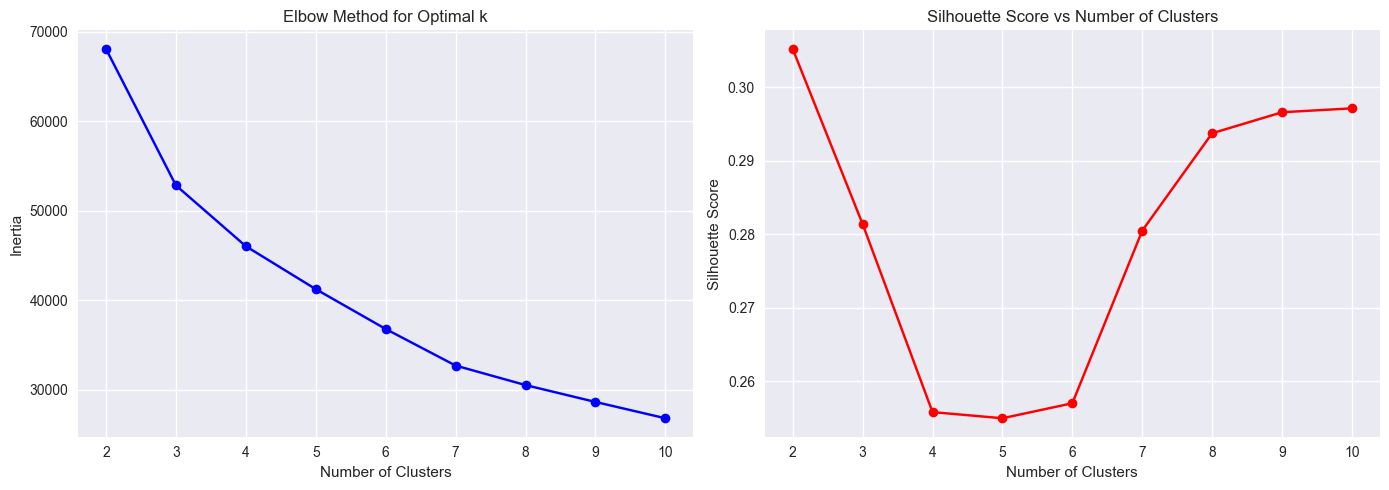
\includegraphics[width=0.9\textwidth]{pics/optimal_clusters.png}
	\caption{تعیین تعداد خوشه‌های بهینه با استفاده از روش \lr{Elbow} و \lr{Silhouette Score}}
	\label{fig:optimal_clusters}
\end{figure}

بر اساس نتایج، تعداد خوشه‌های بهینه برابر با \lr{4} انتخاب شده است که با تعداد کلاس‌های موجود (چهار زبان) مطابقت دارد.

\subsection{الگوریتم‌های خوشه‌بندی}

\subsubsection{\lr{K-Means}}
الگوریتم \lr{K-Means} یکی از ساده‌ترین و پرکاربردترین الگوریتم‌های خوشه‌بندی است. نتایج حاصل از اجرای این الگوریتم با \lr{4} خوشه در جدول \ref{tab:kmeans_results} نمایش داده شده است.

\begin{table}[H]
	\centering
	\caption{نتایج خوشه‌بندی \lr{K-Means}}
	\label{tab:kmeans_results}

	\begin{tabular}{cc}
		\toprule
		معیار & مقدار \\
		\midrule
		\lr{Silhouette Score} & $0.2558$ \\
		\lr{Inertia} & $46053.22$ \\
		\midrule
		تعداد نمونه‌ها در خوشه 0 & 253 \\
		تعداد نمونه‌ها در خوشه 1 & 152 \\
		تعداد نمونه‌ها در خوشه 2 & 92 \\
		تعداد نمونه‌ها در خوشه 3 & 223 \\
		\bottomrule
	\end{tabular}

\end{table}

\subsubsection{\lr{Agglomerative Clustering (Single Link)}}
الگوریتم خوشه‌بندی سلسله‌مراتبی با استفاده از پیوند \lr{Single Link} اجرا شده است. نتایج در جدول \ref{tab:hierarchical_results} نمایش داده شده است.

\begin{table}[H]
	\centering
	\caption{نتایج خوشه‌بندی سلسله‌مراتبی}
	\label{tab:hierarchical_results}

	\begin{tabular}{cc}
		\toprule
		معیار & مقدار \\
		\midrule
		\lr{Silhouette Score} & $0.2103$ \\
		\midrule
		تعداد نمونه‌ها در خوشه 0 & 696 \\
		تعداد نمونه‌ها در خوشه 1 & 3 \\
		تعداد نمونه‌ها در خوشه 2 & 10 \\
		تعداد نمونه‌ها در خوشه 3 & 11 \\
		\bottomrule
	\end{tabular}

\end{table}

همانطور که مشاهده می‌شود، این الگوریتم یک خوشه بزرگ با \lr{696} نمونه و سه خوشه کوچک ایجاد کرده است که نشان‌دهنده مشکل الگوریتم \lr{Single Link} در تشخیص خوشه‌های با اندازه‌های مختلف است.

\subsubsection{\lr{Gaussian Mixture Model (GMM)}}
الگوریتم \lr{GMM} با استفاده از مدل مخلوط گاوسی اجرا شده است. نتایج در جدول \ref{tab:gmm_results} نمایش داده شده است.

\begin{table}[H]
	\centering
	\caption{نتایج خوشه‌بندی \lr{GMM}}
	\label{tab:gmm_results}

	\begin{tabular}{cc}
		\toprule
		معیار & مقدار \\
		\midrule
		\lr{Silhouette Score} & $0.2808$ \\
		\lr{Log Likelhood} & $193744.81$ \\
		\midrule
		تعداد نمونه‌ها در خوشه 0 & 269 \\
		تعداد نمونه‌ها در خوشه 1 & 278 \\
		تعداد نمونه‌ها در خوشه 2 & 88 \\
		تعداد نمونه‌ها در خوشه 3 & 85 \\
		\bottomrule
	\end{tabular}

\end{table}

\subsection{مقایسه الگوریتم‌های خوشه‌بندی}
جدول \ref{tab:clustering_comparison} مقایسه کلی الگوریتم‌های خوشه‌بندی را نشان می‌دهد.

\begin{table}[H]
	\centering
	\caption{مقایسه الگوریتم‌های خوشه‌بندی}
	\label{tab:clustering_comparison}

	\begin{tabular}{lcc}
		\toprule
		الگوریتم & \lr{Silhouette Score} & توزیع خوشه‌ها \\
		\midrule
		\lr{K-Means} & $0.2558$  \\
		\lr{Hierarchical (Single Link)} & $0.2103$  \\
		\lr{GMM} & $0.2808$  \\
		\bottomrule
	\end{tabular}
\end{table}

شکل \ref{fig:clustering_visualization} نمایش بصری نتایج خوشه‌بندی را با استفاده از \lr{PCA} نشان می‌دهد.

\begin{figure}[H]
	\centering
	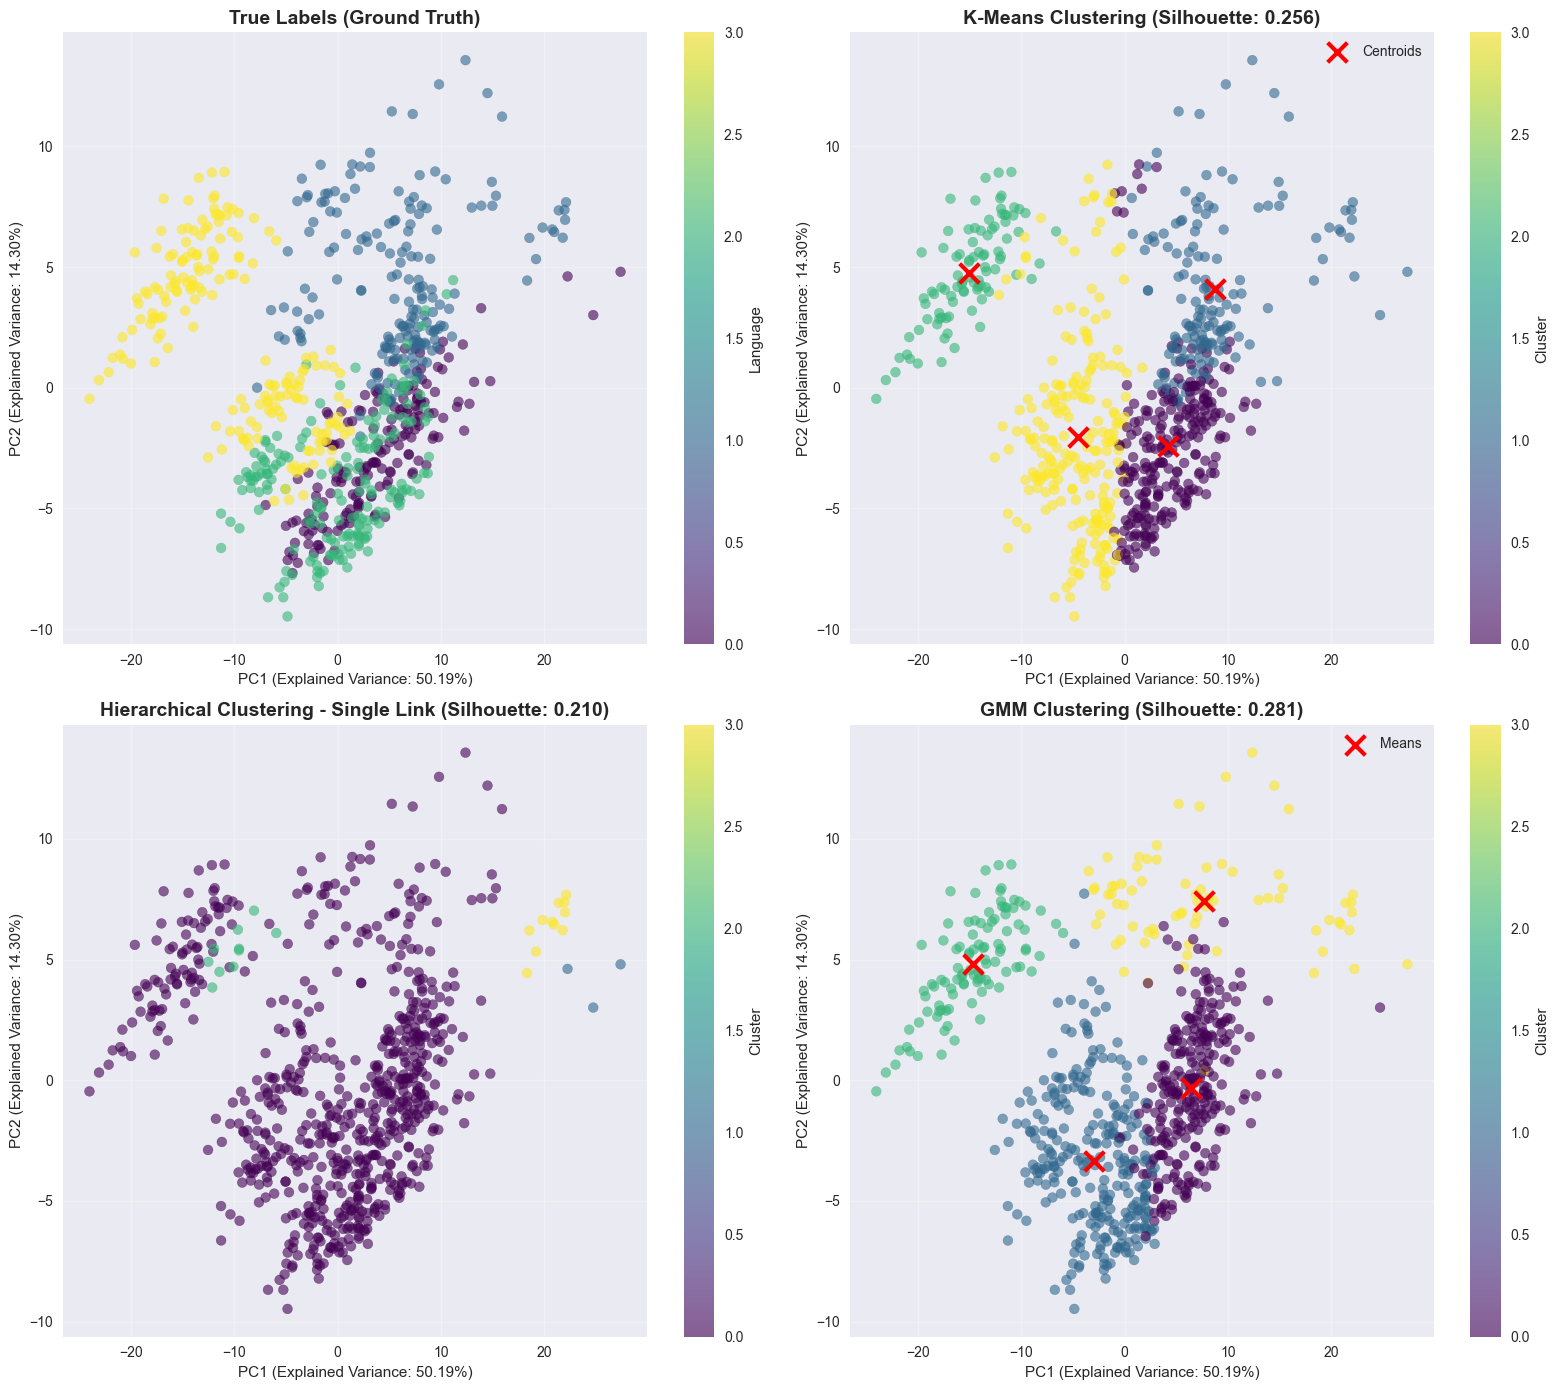
\includegraphics[width=0.9\textwidth]{pics/clustering_visualization.png}
	\caption{نمایش بصری نتایج خوشه‌بندی با استفاده از \lr{PCA}}
	\label{fig:clustering_visualization}
\end{figure}

\section{طبقه‌بندی}

\subsection{تقسیم داده‌ها}
داده‌ها به صورت تصادفی به دو مجموعه آموزش و آزمون تقسیم شده‌اند:
\begin{itemize}
	\item مجموعه آموزش: \lr{576} نمونه (\lr{80\%})
	\item مجموعه آزمون: \lr{144} نمونه (\lr{20\%})
\end{itemize}

توزیع کلاس‌ها در هر دو مجموعه به صورت یکنواخت حفظ شده است.

\subsection{الگوریتم‌های طبقه‌بندی}

\subsubsection{\lr{K-Nearest Neighbors (KNN)}}
الگوریتم \lr{KNN} با استفاده از همسایگان نزدیک برای طبقه‌بندی استفاده شده است.

\subsubsection{\lr{Support Vector Machine (SVM)}}
الگوریتم \lr{SVM} با استفاده از کرنل مناسب برای طبقه‌بندی چندکلاسه استفاده شده است.

\subsubsection{\lr{Random Forest}}
الگوریتم \lr{Random Forest} با استفاده از مجموعه‌ای از درخت‌های تصمیم‌گیری اجرا شده است.

\subsubsection{\lr{Neural Network (MLP)}}
شبکه عصبی چندلایه (\lr{MLP}) با استفاده از \lr{MLPClassifier} اجرا شده است.

\subsection{نتایج طبقه‌بندی}
نتایج حاصل از اجرای الگوریتم‌های مختلف در جدول \ref{tab:classification_results} نمایش داده شده است.

\begin{table}[H]
	\centering
	\caption{نتایج کلی طبقه‌بندی}
	\label{tab:classification_results}
	\begin{latin}
	\begin{tabular}{lc}
		\toprule
		الگوریتم & دقت (Accuracy) \\
		\midrule
		KNN & 0.9722 \\
		SVM & 0.9861 \\
		Random Forest & 0.9861 \\
		Neural Network & 0.9722 \\
		\bottomrule
	\end{tabular}
	\end{latin}
\end{table}

جدول \ref{tab:detailed_metrics} معیارهای تفصیلی شامل \lr{Precision}، \lr{Recall} و \lr{F1-Score} را برای هر الگوریتم نشان می‌دهد.

\begin{table}[H]
	\centering
	\caption{معیارهای تفصیلی طبقه‌بندی}
	\label{tab:detailed_metrics}
	\resizebox{\textwidth}{!}{%
	\begin{latin}
	\begin{tabular}{lccccccc}
		\toprule
		الگوریتم & دقت & Macro Precision & Macro Recall & Macro F1 & Weighted Precision & Weighted Recall & Weighted F1 \\
		\midrule
		KNN & 0.9722 & 0.9737 & 0.9722 & 0.9722 & 0.9737 & 0.9722 & 0.9722 \\
		SVM & 0.9861 & 0.9865 & 0.9861 & 0.9861 & 0.9865 & 0.9861 & 0.9861 \\
		Random Forest & 0.9861 & 0.9865 & 0.9861 & 0.9860 & 0.9865 & 0.9861 & 0.9860 \\
		Neural Network & 0.9722 & 0.9737 & 0.9722 & 0.9722 & 0.9737 & 0.9722 & 0.9722 \\
		\bottomrule
	\end{tabular}%
	\end{latin}
	}
\end{table}

شکل \ref{fig:classification_metrics} نمایش بصری معیارهای مختلف را برای الگوریتم‌های مختلف نشان می‌دهد.

\begin{figure}[H]
	\centering
	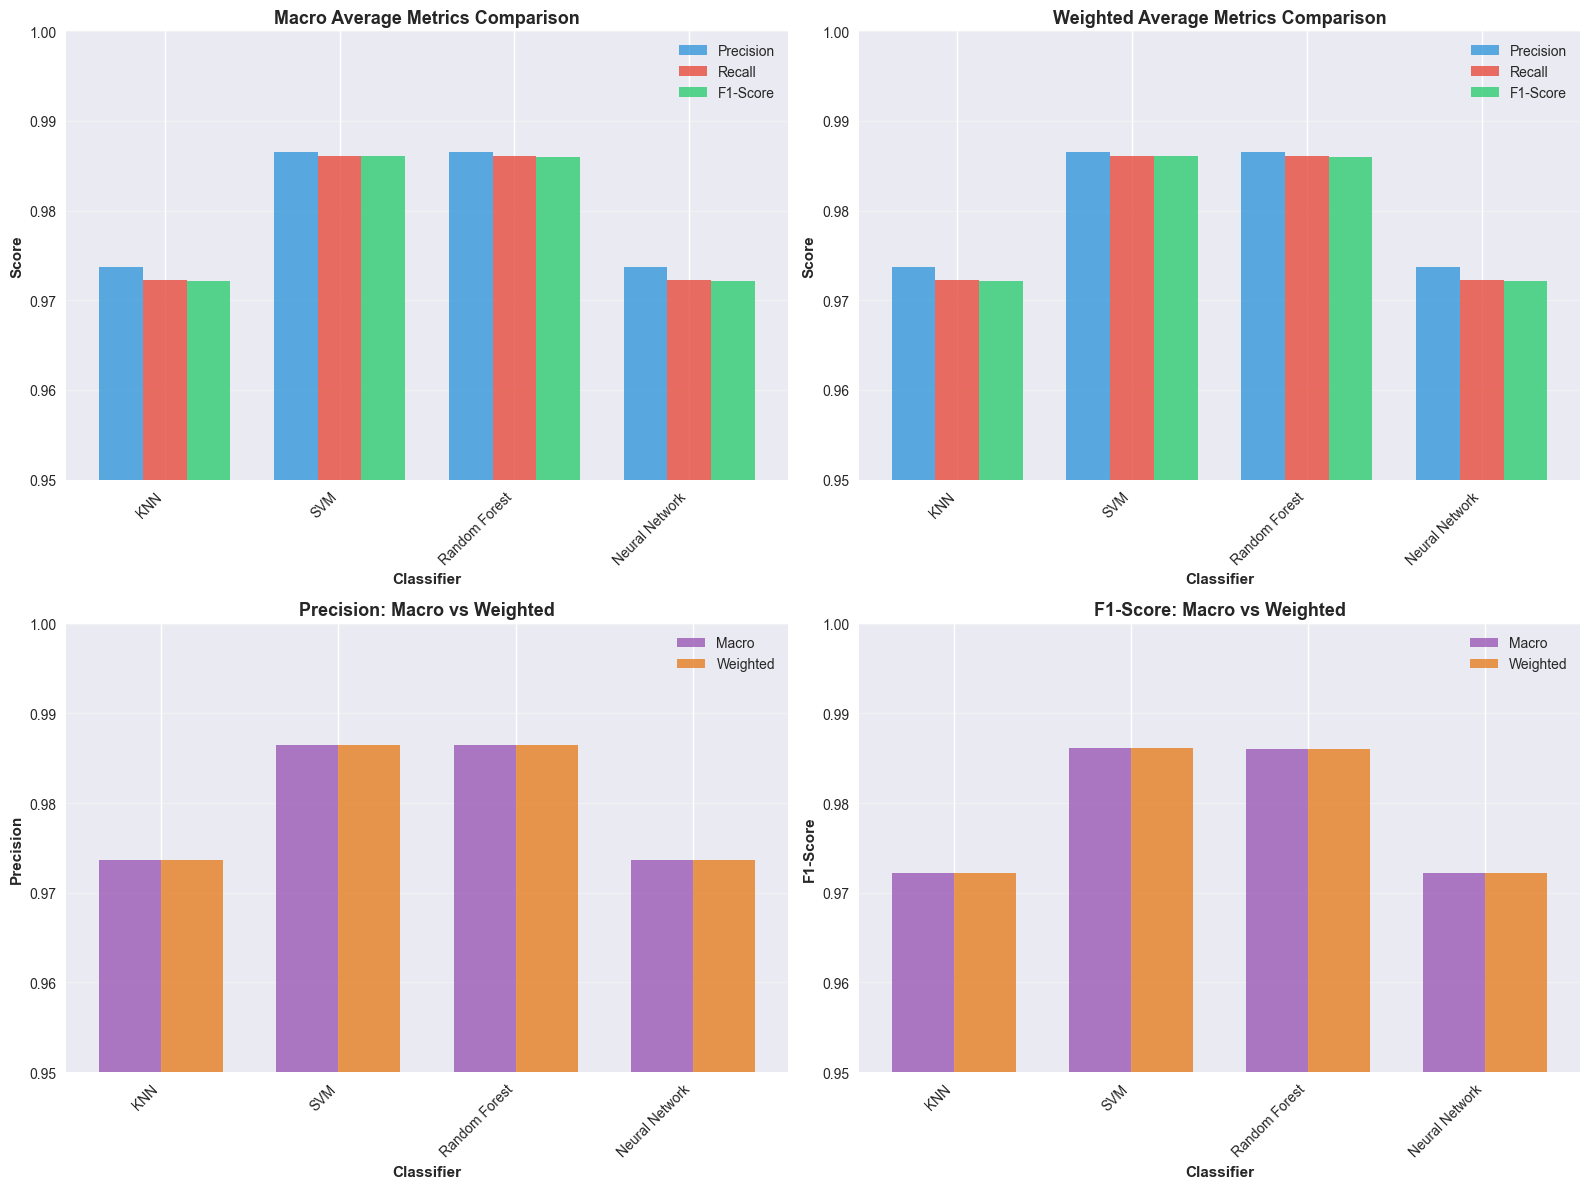
\includegraphics[width=0.9\textwidth]{pics/classification_metrics.png}
	\caption{مقایسه معیارهای مختلف طبقه‌بندی}
	\label{fig:classification_metrics}
\end{figure}

\subsection{ماتریس درهم‌ریختگی}
ماتریس‌های درهم‌ریختگی برای هر الگوریتم در شکل \ref{fig:confusion_matrices} نمایش داده شده‌اند.

\begin{figure}[H]
	\centering
	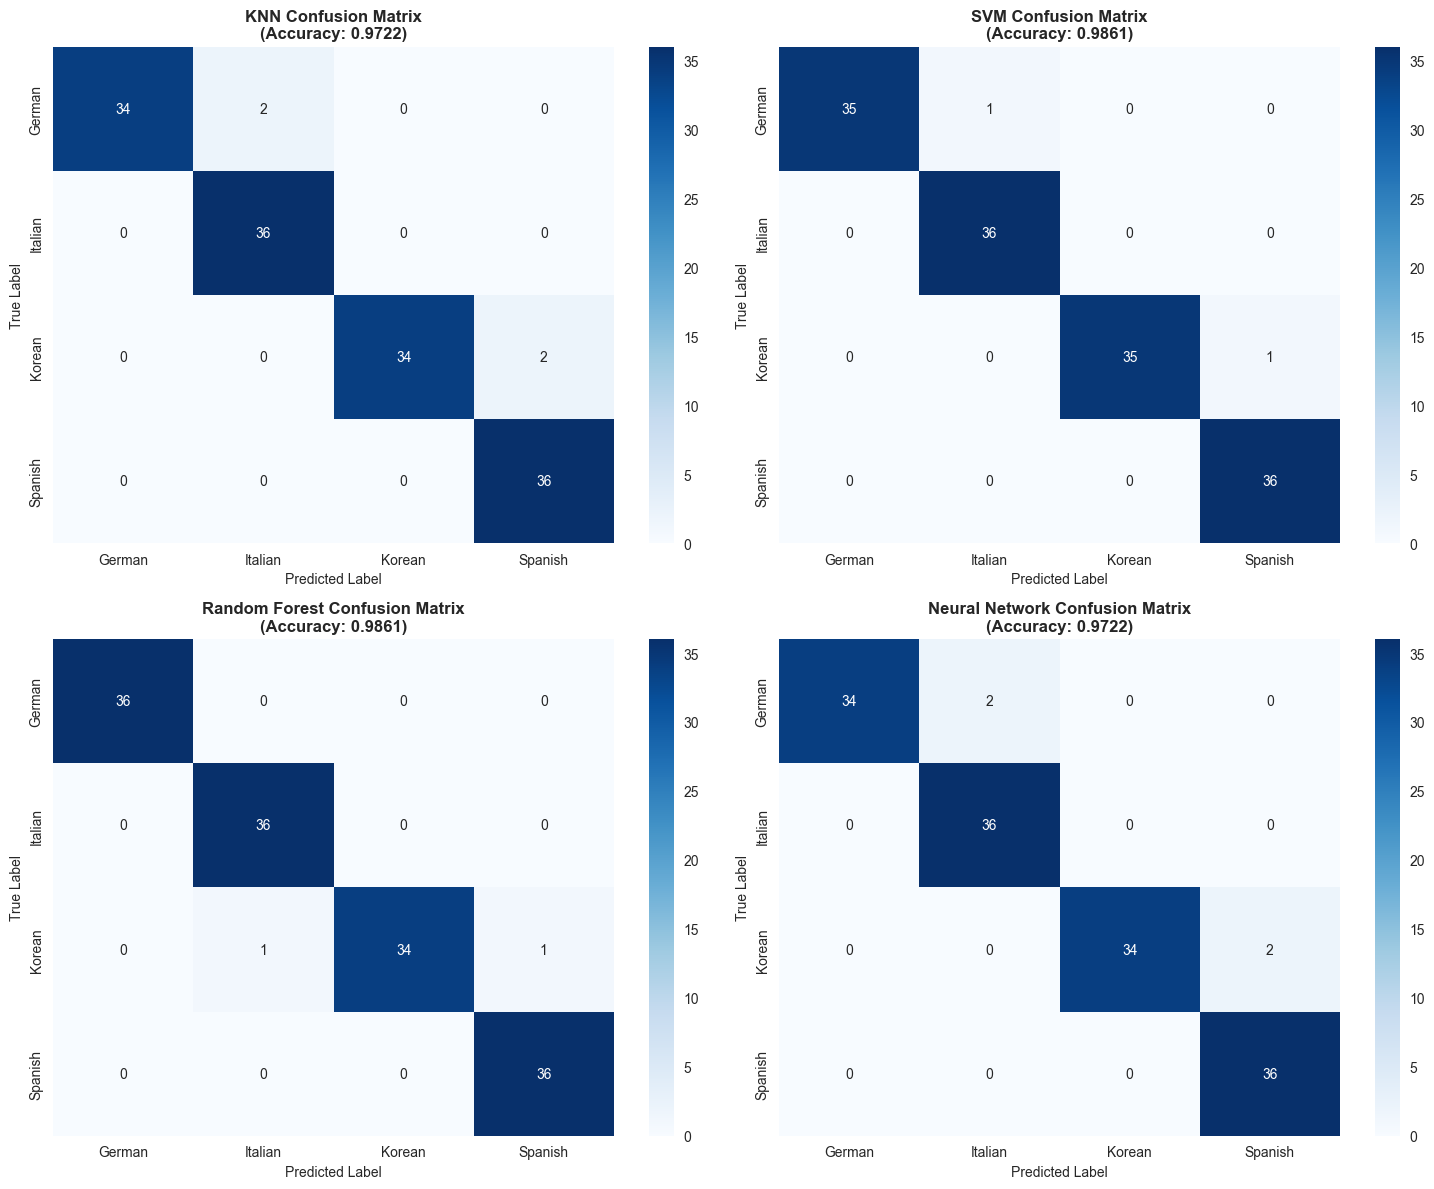
\includegraphics[width=0.9\textwidth]{pics/confusion_matrices.png}
	\caption{ماتریس‌های درهم‌ریختگی برای الگوریتم‌های مختلف}
	\label{fig:confusion_matrices}
\end{figure}

\section{بحث و نتیجه‌گیری}

\subsection{نتایج خوشه‌بندی}
از بین الگوریتم‌های خوشه‌بندی مورد استفاده، \lr{K-Means} بهترین عملکرد را با \lr{Silhouette Score} برابر با \lr{0.2558} داشته است. این الگوریتم توزیع متعادلی از نمونه‌ها در خوشه‌های مختلف ایجاد کرده است. الگوریتم \lr{Hierarchical} با \lr{Single Link} عملکرد ضعیف‌تری داشته و یک خوشه بزرگ با اکثریت نمونه‌ها ایجاد کرده است.

\subsection{نتایج طبقه‌بندی}
همه الگوریتم‌های طبقه‌بندی عملکرد بسیار خوبی داشته‌اند و دقت بالای \lr{97\%} را نشان داده‌اند. \lr{SVM} و \lr{Random Forest} با دقت \lr{98.61\%} بهترین عملکرد را داشته‌اند. \lr{KNN} و \lr{Neural Network} نیز با دقت \lr{97.22\%} عملکرد بسیار خوبی داشته‌اند.

تفاوت‌های جزئی در معیارهای \lr{Precision}، \lr{Recall} و \lr{F1-Score} نشان می‌دهد که همه الگوریتم‌ها به خوبی قادر به تشخیص و تمایز بین زبان‌های مختلف هستند.

\subsection{نتیجه‌گیری نهایی}
نتایج نشان می‌دهد که ویژگی‌های استخراج شده (\lr{MFCC} و \lr{Mel Spectrogram}) برای تشخیص زبان مناسب هستند و الگوریتم‌های یادگیری ماشین قادر به استفاده مؤثر از این ویژگی‌ها هستند. در بین الگوریتم‌های طبقه‌بندی، \lr{SVM} و \lr{Random Forest} بهترین عملکرد را داشته‌اند و می‌توانند برای کاربردهای عملی استفاده شوند. برای افزایش دقت می‌توان تعداد ویژگی‌ها را بیشتر کرد و از مدل‌هایی که از این نکته بهره می‌برند، مثل شبکه عصبی استفاده کرد تا دقت بالاتری گرفت.

خوشه‌بندی حتی در بهترین حالت هم نمی‌تواند به عنوان معیار خوبی برای تشخیص زبان‌ها باشد. ولی می‌توان از آن برای سنجش شباهت زبان‌ها به هم استفاده کرد. 
	
	چون حساب کردن متریک‌ها به داده خروجی نیاز دارد، در همان نوتبوک‌های 
	\lr{classification}
	و
	\lr{clustering}
	متریک‌ها حساب شدند.
\end{document}